\documentclass[a4paper]{article}

\input ../header
\usepackage{minted}
\usepackage[np]{numprint}
\usepackage{lscape}
\usepackage{afterpage}
\usepackage{hyperref}
\usepackage{gensymb}

\setlength{\multicolsep}{2pt}

% Commandes pour cacher/révéler du texte facilement à l'aide d'un booléen
\usepackage{xstring}
\usepackage{ifthen}

\newboolean{reveal}
\setboolean{reveal}{false}

\newlength{\stextwidth} % une nouvelle longueur

\newcommand\x{6}

\newcommand{\guess}[1]{\ifthenelse{\boolean{reveal}}{{\color{red}#1}}{\settowidth{\stextwidth}{#1}\makebox[\stextwidth]{\dotfill}}}

\newcommand{\guessmath}[1]{\ifthenelse{\boolean{reveal}}{\textcolor{red}{#1}}{\settowidth{\stextwidth}{$#1$}\makebox[1.9\stextwidth]{\dotfill}}}

\newcommand{\guessmathbin}[1]{\ifthenelse{\boolean{reveal}}{\mathbin{\color{red}#1}}{\settowidth{\stextwidth}{$#1$}\makebox[2\stextwidth]{\dotfill}}}

\begin{document}

\title{Chapitre 6 -- Géolocalisation}

\pagestyle{empty}

\date{}
\author{}

\maketitle{}

\thispagestyle{empty}
\noindent\textbf{Activité 3}\hfill{}\textbf{Trilatération}
\smallskip
\hrule
\medskip

\begin{enumerate}
  \item \textbf{Calculer une distance} 

    Un satellite envoie un signal voyageant à la vitesse de la lumière à un récepteur GPS. Ce signal contient les informations suivantes : 
    \begin{center}
      \verb|Date d'émission : 14 Avril 2021 @ 18h 27min 04s 123ms GMT-10|
    \end{center}

    La date affichée sur le récepteur GPS au moment de la réception du signal est : 
    \begin{center}
      \verb|Date : 14 Avril 2021 @ 18h 27min 04s 243ms GMT-10|
    \end{center}

    Calculer la distance qui sépare le récepteur GPS du satellite.\rep{4}

    %	{\color{blue}
    %		D'après l'énoncé, le signal a mis $120$ ms pour atteindre le récepteur GPS. 
    %		
    %		Comme la vitesse du signal est de $\np{300 000}$ km/s soit $\np{300}$ km/ms
    %		
    %		On en déduit donc que la distance $d$ qui sépare le satellite du récepteur GPS est : 
    %		
    %		\[d = 300 \times 120 = \np{36000} \mbox{\ km}\]
    %	}

  \item \textbf{Trouver des coordonnées}
    \begin{itemize}
      \item[$\bullet$] Les points $A(-2\,;\,4)$, $B(3\,;\,1)$ et $C(2\,;\,5)$ représentent la position de trois satellites. 
      \item[$\bullet$] Le point $M(x\,;\,y)$ correspond à la position du récepteur GPS. 
      \item[$\bullet$] Les cercles $\mathcal{C}_A$, $\mathcal{C}_B$ et $\mathcal{C}_C$ ont pour rayons respectifs :

	\[AM = \sqrt{10},\ BM = \sqrt{8} \mbox{ et } CM = \sqrt{5}\]

	\begin{center}
	  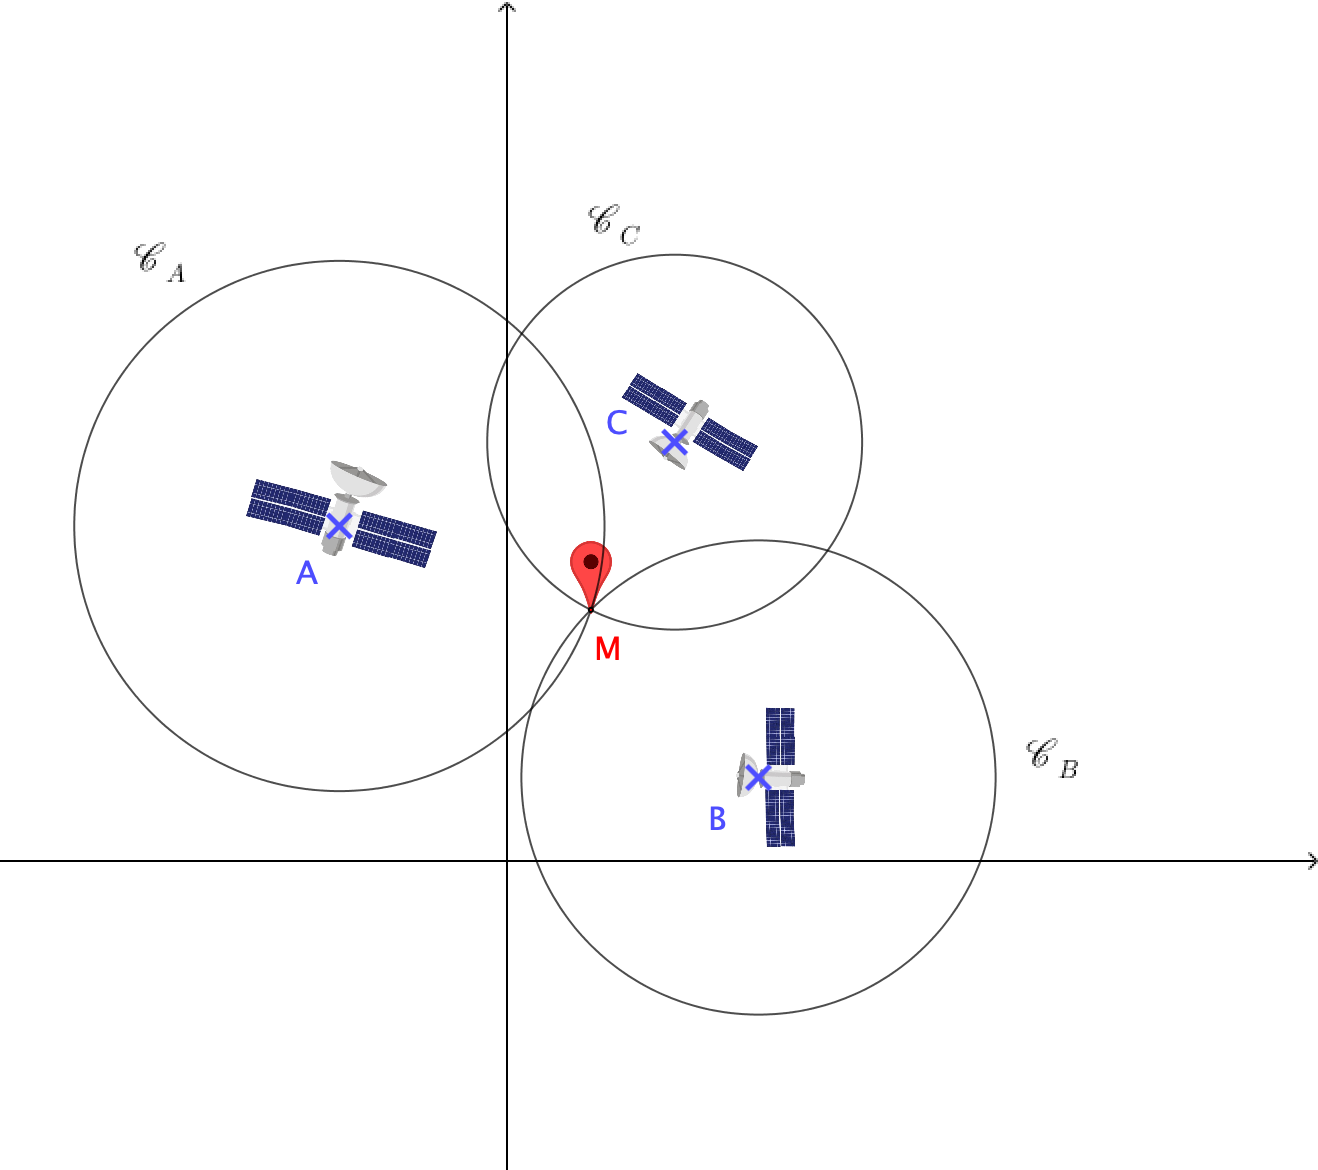
\includegraphics[width = 14cm]{trilateration.png}
	\end{center}

	\pagebreak

	L'objectif de ce qui suit est de déterminer la position du point $M$ dans le plan.

    \end{itemize}

    \begin{enumerate}
      \item La distance $AM^2$ en fonction des coordonnées $x$ et $y$ du point $M$ est donnée par : 

	\[AM^2 = x^2+y^2+4x-8y+20\]

	Justifier cette égalité.\rep{8}

      \item Exprimer $BM^2$ et $CM^2$ en fonction des coordonnées $x$ et $y$ du point $M$.\rep{8}

	  %	{\color{blue}
	  %	
	  %	\[
	  %	\renewcommand\arraystretch{2}
	  %	\begin{array}{lcl}
	  %		BM^2 &  = & (x-x_B)^2+(y-y_B)^2 = (x-3)^2+(y-1)^2 \\
	  %		& =  & x^2-6x+9+y^2-2y+1 = x^2+y^2-6x-2y+10 \\
	  %	\end{array}\]
	  %	
	  %	\[
	  %	\renewcommand\arraystretch{2}
	  %	\begin{array}{lcl}
	  %		CM^2 &  = & (x-x_C)^2+(y-y_C)^2 = (x-2)^2+(y-5)^2 \\
	  %		& =  & x^2-4x+4+y^2-10y+25 = x^2+y^2-4x-10y+29 \\
	  %	\end{array}\]
	  %		
	  %	}

	\item Justifier que pour trouver les coordonnées du point $M$, il suffit de résoudre le système suivant :

	  \[
	    (S) : \left\{
	      \begin{aligned}
		5x - 3y +4 &= 0 \\
		4x + y -7  &= 0 \\
	    \end{aligned}\right.
	  \]

	  \dotfill\rep{7}

	\item Déterminer les coordonnées de $M$.\rep{16}

	  %	{\color{blue}
	  %	
	  %		\[
	  %		\renewcommand\arraystretch{1.25}
	  %		\begin{array}{lcl}
	  %	(S) : \left\{
	  %	\begin{array}{rcl}
	  %	5x - 3y +4 & = & 0 \\
	  %	4x + y -7  & = & 0 \\
	  %	\end{array}\right.
	  %	&
	  %	\Leftrightarrow 
	  %	&
	  %	\left\{
	  %	\begin{array}{rcl}
	  %	5x - 3y +4 & = & 0 \\
	  %	y  & = & -4x + 7 \\
	  %	\end{array}\right.\\
	  %	&&\\
	  %	
	  %	&
	  %	\Leftrightarrow 
	  %	&
	  %	\left\{
	  %	\begin{array}{rcl}
	  %	5x - 3(-4x+7) +4 & = & 0 \\
	  %	y  & = & -4x + 7 \\
	  %	\end{array}\right.\\
	  %	
	  %	&& \\
	  %		&
	  %	\Leftrightarrow 
	  %	&
	  %	\left\{
	  %	\begin{array}{rcl}
	  %	17x - 17 & = & 0 \\
	  %	y  & = & -4x + 7 \\
	  %	\end{array}\right.\Leftrightarrow
	  %	\left\{
	  %	\begin{array}{rcl}
	  %	x& = & 1 \\
	  %	y  & = & -4x + 7 \\
	  %	\end{array}\right.\\
	  %	
	  %	&&\\
	  %	
	  %	&
	  %	\Leftrightarrow 
	  %	&
	  %	\left\{
	  %	\begin{array}{rcl}
	  %	x & = & 1 \\
	  %	y  & = & 3 \\
	  %	\end{array}\right.\\
	  %	
	  %	\end{array}
	  %	\] 
	  %	
	  %	Le point $M$ a donc pour coordonnées $(1\,;\,3)$. 
	  %	}
      \end{enumerate}
    \item \textbf{ Et l'altitude ?}

      Dans la représentation de la question précédente, nous obtenons les coordonnées dans le plan du point $M$. Cependant, la localisation GPS permet de situer le récepteur GPS dans l'espace. 

      Que faudrait-il utiliser à la place des cercles pour obtenir une géolocalisation dans l'espace ? \rep{3}

      % {\color{blue} Pour situer le récepteur GPS dans l'espace, il faudrait considérer l'intersection de 3 sphères au lieu de l'intersection de 3 cercles.
      % 
      % }

  \end{enumerate}
\end{document}
